%----------------------------------------------------------------------------------------
%	PACKAGES AND THEMES
%----------------------------------------------------------------------------------------
\documentclass[aspectratio=169,xcolor=dvipsnames]{beamer}
\usetheme{SimplePlus}
\newcommand{\vect}[1]{\boldsymbol{#1}}


\usepackage{hyperref}
\usepackage{graphicx} % Allows including images
\usepackage{booktabs} % Allows the use of \toprule, \midrule and \bottomrule in tables

%----------------------------------------------------------------------------------------
%	TITLE PAGE
%----------------------------------------------------------------------------------------

\title[short title]{CUDA Implementation of Position Based Fluids} % The short title appears at the bottom of every slide, the full title is only on the title page
\subtitle{CSC417 Course Project}

\author[Qingyuan.Sheldon] {Qingyuan Qie, Changlin Su}

\institute[UofT] % Your institution as it will appear on the bottom of every slide, may be shorthand to save space
{
    Department of Computer Science \\
    University of Toronto
}
\date{\today} % Date, can be changed to a custom date


%----------------------------------------------------------------------------------------
%	PRESENTATION SLIDES
%----------------------------------------------------------------------------------------

\begin{document}

\begin{frame}
    % Print the title page as the first slide
    \titlepage
\end{frame}

% \begin{frame}{Overview}
%     % Throughout your presentation, if you choose to use \section{} and \subsection{} commands, these will automatically be printed on this slide as an overview of your presentation
%     \tableofcontents
% \end{frame}

\begin{frame}{Enforcing incompressibility}
    For particle $i$ at position $p_i$, we compute the density of the fluid around particle $i$ using the estimator:
    
  $\rho_{F(i)} = \sum_{j \in F(i)} m_j W_{poly6}(\vect{p}_i - \vect{p}_j, h)$
    
\end{frame}

\begin{frame}{Enforcing incompressibility}
    For particle $i$ at position $\vect{p}_i$, we compute the density of the fluid around particle $i$ using the estimator:
    
  $\rho_{i} = \sum_{j \in F(i)} m_j W_{poly6}(\vect{p}_i - \vect{p}_j, h)$ \\[2ex]
  Then we have the constant density constraint:

  $C_i(\vect{p}) = \frac{\rho_i}{\rho_0} - 1$ \\[2ex]

\end{frame}

\begin{frame}{Enforcing incompressibility}
    For particle $i$ at position $\vect{p}_i$, we compute the density of the fluid around particle $i$ using the estimator:
    
  $\rho_{i} = \sum_{j \in F(i)} m_j W_{poly6}(\vect{p}_i - \vect{p}_j, h)$ \\[2ex]
  Then we have the constant density constraint:

  $C_i(\vect{p}) = \frac{\rho_i}{\rho_0} - 1$ \\[2ex]

  And we want to compute a position correction $\Delta \vect{p}$, such that:

  $C(\vect{p} + \Delta \vect{\vect{p}}) = 0$
    
\end{frame}

\begin{frame}{Position Update from Solving Incompressibility}
    For particle $i$ at position $\vect{p}_i$, we have,

    $  \lambda_i = -\frac{C_i(\vect{p})}{\sum_k |\nabla_{\vect{p}_k} C_i|^2}$ \\[2ex]
    
\end{frame}

\begin{frame}{Position Update from Solving Incompressibility}
    For particle $i$ at position $\vect{p}_i$, we have,

    $  \lambda_i = -\frac{C_i(\vect{p})}{\sum_k |\nabla_{\vect{p}_k} C_i|^2}$ \\[2ex]

    Then the position correction $\Delta \vect{p}_i$ including affect from neighboring particles is,

    $\Delta \vect{p}_i = \frac{1}{\rho_0} \sum_j (\lambda_i + \lambda_j) \nabla W(\vect{p}_i - \vect{p}_j , h)$ \\[2ex]
    
\end{frame}

\begin{frame}{Position Update from Solving Incompressibility}
    For particle $i$ at position $\vect{p}_i$, we have,

    $  \lambda_i = -\frac{C_i(\vect{p})}{\sum_k |\nabla_{\vect{p}_k} C_i|^2}$ \\[2ex]

    Then the position correction $\Delta \vect{p}_i$ including affect from neighboring particles is,

    $\Delta \vect{p}_i = \frac{1}{\rho_0} \sum_j (\lambda_i + \lambda_j) \nabla W(\vect{p}_i - \vect{p}_j , h)$ \\[2ex]

    And the position update is,

    $\vect{p}_i^* = \vect{p}_i + \Delta \vect{p}_i$

    
\end{frame}

\begin{frame}{Simulation Step}
    \begin{figure}
    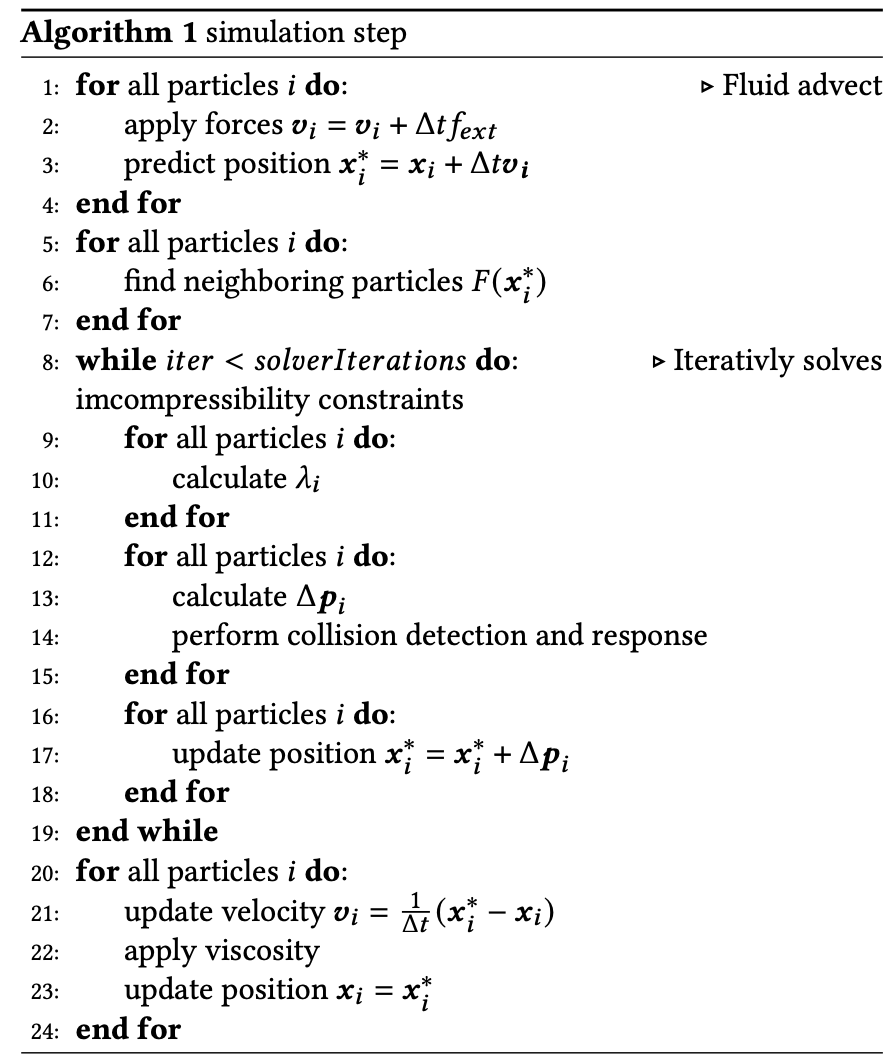
\includegraphics[width=0.4\linewidth]{../image/algorithm.png}
    \end{figure}

\end{frame}

\begin{frame}{Performance of Implementation}
    \begin{figure}
        \centering
        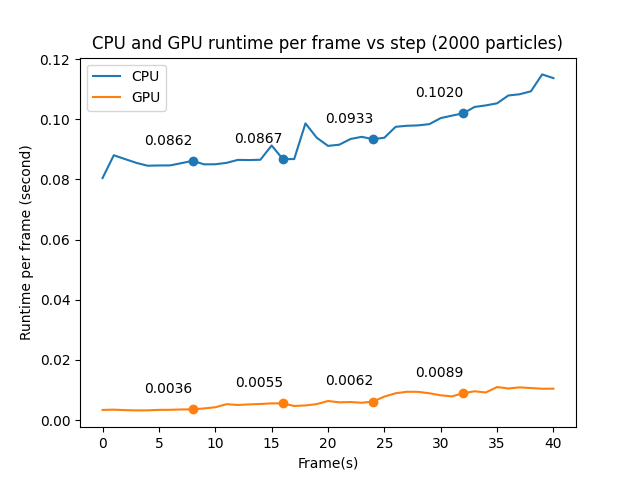
\includegraphics[width=0.6\linewidth]{../image/cpu-gpu-comprasion.png}
        \caption{Performance Comparison between CPU ans GPU, 2k particles}
    \end{figure}

\end{frame}


\begin{frame}{Performance of CUDA Implementation}
    \begin{center}
        \begin{tabular}{| c | c | c |}
          \hline
          Particle Count & Time per Frame & Frame per Second(fps)  \\
          \hline
          2k & 0.006s & 166fps \\
          \hline
          12k & 0.01s &  100fps \\
          \hline
          27k & 0.021s & 47.6fps \\
          \hline
          80k & 0.064 & 15.6fps \\
          \hline
        \end{tabular}
    \end{center}
\end{frame}


\end{document}